% !TEX program = xelatex
\documentclass[10pt,letterpaper,twocolumn]{article}

% === PAGE ===
\usepackage[top=0.75in,bottom=0.75in,left=0.75in,right=0.75in,footskip=12pt]{geometry}

% === FONTS ===
\usepackage{fontspec}
\usepackage{unicode-math}
\setmainfont{Latin Modern Roman}[
  Extension=.otf,
  UprightFont=lmroman10-regular,
  BoldFont=lmroman10-bold,
  ItalicFont=lmroman10-italic,
  BoldItalicFont=lmroman10-bolditalic,
]
\setsansfont{Latin Modern Sans}[
  Extension=.otf,
  UprightFont=lmsans10-regular,
  BoldFont=lmsans10-bold,
  ItalicFont=lmsans10-oblique,
  BoldItalicFont=lmsans10-boldoblique,
]
\setmonofont{Latin Modern Mono}[
  Extension=.otf,
  UprightFont=lmmono10-regular,
  ItalicFont=lmmono10-italic,
  Scale=0.85,
]
% Match the Keymaps paper: YWFT Processing appears only in the title.
\newfontfamily\acbold{ywft-processing-bold}[
  Path=../../system/public/type/webfonts/,
  Extension=.ttf
]

% === PACKAGES ===
\usepackage{xcolor}
\usepackage{titlesec}
\usepackage{enumitem}
\usepackage{booktabs}
\usepackage{tabularx}
\usepackage{fancyhdr}
\usepackage{hyperref}
\usepackage{xurl}
\usepackage{graphicx}
\graphicspath{{./}{figures/}}
\usepackage{ragged2e}
\usepackage{microtype}
\usepackage[font=footnotesize]{caption}
\usepackage{natbib}
\usepackage{multicol}
\usepackage{tikz}
\usetikzlibrary{arrows.meta,calc,positioning}

% === COLORS ===
\definecolor{acpink}{RGB}{180,72,135}
\definecolor{acpurple}{RGB}{120,80,180}
\definecolor{acdark}{RGB}{64,56,74}
\definecolor{acgray}{RGB}{119,119,119}
\definecolor{acblue}{RGB}{42,100,212}

% === LINKS ===
\hypersetup{
  colorlinks=true,
  linkcolor=acpurple,
  urlcolor=acpurple,
  citecolor=acpurple,
  pdfauthor={@jeffrey},
  pdftitle={Pieces Not Programs: The Piece as a Versioned, Performable Unit of Creative Computing},
}

% === SECTIONS ===
\titleformat{\section}
  {\normalfont\bfseries\normalsize\uppercase}
  {\thesection.}
  {0.5em}
  {}
\titlespacing{\section}{0pt}{1.2em}{0.3em}
\titleformat{\subsection}
  {\normalfont\bfseries\small}
  {\thesubsection}
  {0.5em}
  {}
\titlespacing{\subsection}{0pt}{0.8em}{0.2em}

% === RUNNING MATTER ===
\pagestyle{fancy}
\fancyhf{}
\renewcommand{\headrulewidth}{0pt}
\fancyfoot[C]{\footnotesize\thepage}
\setlist[itemize]{nosep,leftmargin=1.2em,itemsep=0.1em}
\setlist[enumerate]{nosep,leftmargin=1.2em}
\setlength{\columnsep}{1.8em}
\setlength{\parindent}{1em}
\setlength{\parskip}{0.3em}
\tolerance=800
\emergencystretch=1em
\hyphenpenalty=50

\newcommand{\acdot}{{\color{acpink}.}}
\newcommand{\ac}{Aesthetic{\acdot}Computer}
\newcommand{\code}[1]{\texttt{#1}}
\newcommand{\datum}[1]{\textbf{\color{acdark}#1}}
\newcommand{\coverplate}{%
  \begin{tikzpicture}
    \node[inner sep=0pt,outer sep=0pt,rounded corners=18pt,fill=acpink!6]
      {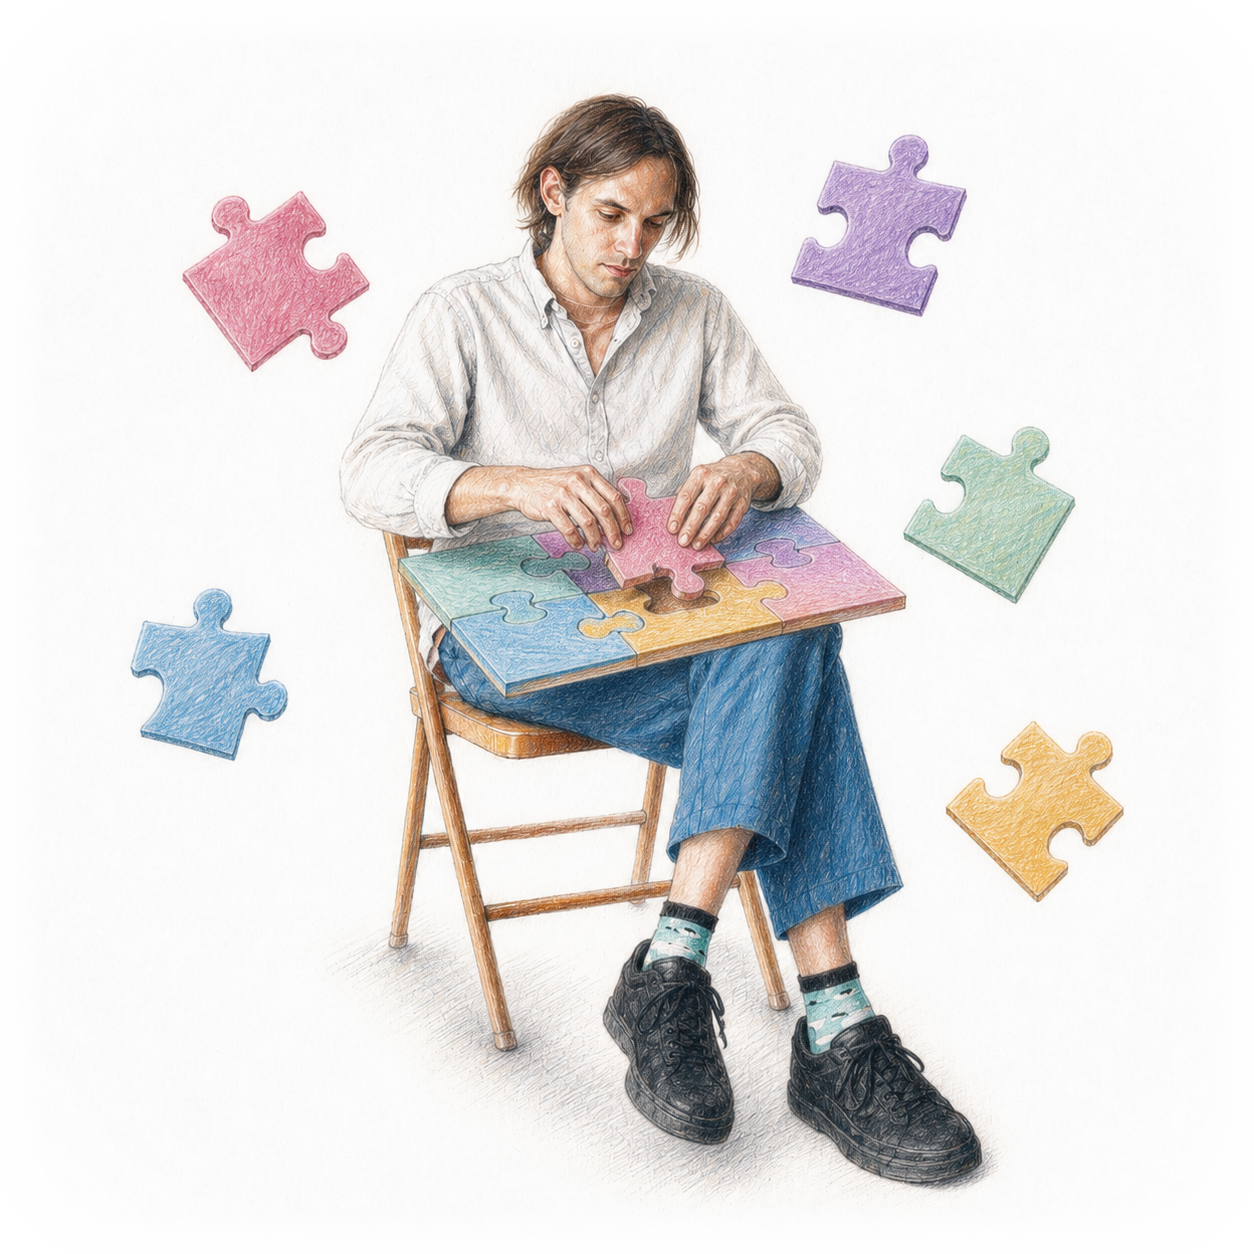
\includegraphics[width=0.66\textwidth]{figures/cover-puzzle-masked}};
  \end{tikzpicture}%
}

% Version macros are stamped by papers/cli.mjs. The fallback keeps a manual
% xelatex build working before the papermill has generated version.tex.
\InputIfFileExists{version}{}{%
  \providecommand{\paperhash}{dev}\providecommand{\paperrev}{?}}

% Cover language bar, matching Keymaps. These are sibling editions, not
% language names, so the Latin-only cover font can render the row everywhere.
\newcommand{\plang}[2]{\href{https://papers.aesthetic.computer/pieces-not-programs-26-arxiv#2.pdf}{\color{acgray}#1}}
\newcommand{\planghere}[1]{{\bfseries\color{acpink}#1}}
\newcommand{\plangsep}{{\color{acgray!60}\,\textperiodcentered\,}}

\begin{document}

\twocolumn[{%
\begin{center}
{\acbold\fontsize{28pt}{32pt}\selectfont\color{acdark} Pieces Not Programs}\par
\vspace{0.45em}
\coverplate\par
\vspace{0.35em}
{\itshape\fontsize{14.5pt}{17pt}\selectfont\color{acpink} The Piece as a Versioned, Performable Unit of Creative Computing}\par
\vspace{0.5em}
{\small\color{acgray} \href{https://prompt.ac/@jeffrey}{@jeffrey} \,\textperiodcentered\, Aesthetic{\acdot}Computer \,\textperiodcentered\, ORCID \href{https://orcid.org/0009-0007-4460-4913}{0009-0007-4460-4913}}\par
\vspace{0.45em}
{\footnotesize\sffamily\planghere{EN}\plangsep\plang{DA}{-da}\plangsep\plang{ES}{-es}\plangsep\plang{ZH}{-zh}\plangsep\plang{JA}{-ja}}\par
\vspace{0.55em}
{\color{acpink}\rule{\textwidth}{1.2pt}}
\vspace{0.5em}
\end{center}

\begin{quote}
\small\noindent\textbf{Abstract.}
\ac{} calls an interactive work a \emph{piece}. The term once described a compact browser program; the August 2026 monorepo shows a larger object. Its 477 built-in entry files include musical instruments, drawing tools, multiplayer worlds, media decks, prompts, and containers. Forty-one percent of the JavaScript entries import shared modules; some depend on authoritative servers; the loader also adapts KidLisp, p5-style JavaScript, and Lua. ``One file, one piece'' is therefore no longer an implementation fact. I define the piece instead as a four-part contract: an authored entry, a named address, a performance instance governed by lifecycle hooks, and a durable record of source, attribution, media, and runs. A piece may execute unchanged in the browser, Electron, or a standalone pack, or persist by contract through a native port. Repository and Platter evidence shows how this unit organizes authorship, composition, security, observability, and return. The contribution is not a synonym for \emph{program}, but a unit of analysis for software whose identity must survive execution, revision, and performance.
\end{quote}
\vspace{0.5em}
}]

\section{An Entry, Not a Container}

The smallest public instruction for making something in \ac{} is still simple: write one \code{.mjs} or \code{.lisp} file, drag or save it into the runtime, and issue \code{publish}. The result receives a path. A built-in work such as \code{notepat} resolves at \code{aesthetic.computer/notepat}; a published work resolves beneath an author's handle, such as \code{@bash/hub}. The \code{source} command returns code for study or revision. This is why \ac{} calls the work a \emph{piece}: it has a name, an author, repeatable performances, and variants.

The earlier version of this paper treated that entry file as the whole object. The monorepo no longer permits that simplification. At commit \code{c65015fe25}, 188 of 455 JavaScript piece entries import shared modules. \code{arena.mjs} shares movement physics with an authoritative session server; thin audiovisual pieces import a common \code{pads.mjs} engine; \code{prompt.mjs} is roughly ten thousand lines and imports other pieces and libraries. One file remains the front door, not the building~\citep{acrepo2026}.

This distinction repairs the title's rhetoric. A piece is not the opposite of a program. It is implemented by programs. \emph{Program} names executable instructions and their dependency graph; \emph{piece} names the authored, addressable work that persists while those instructions change. Tests, correctness, maintenance, and security remain necessary. The artistic term identifies a different boundary.

\section{Related Creative Units}

Creative-computing systems have repeatedly renamed their unit of work. Processing's \emph{sketch} imports provisional drawing practice into the IDE~\citep{reas2007processing}. Max's \emph{patch} names both a spatial dataflow graph and something continually changed while live~\citep{puckette1988patcher,puckette1996pure}. Smalltalk's \emph{image} is a persistent object world rather than a source bundle~\citep{kay1977personal}. Live coding treats source as a changing performance condition rather than a prelude to a finished executable~\citep{blackwell2022livecoding}.

The \emph{piece} takes a different cut through the same field. From music it inherits the distinction between score and performance: no rendition exhausts the work, but renditions remain recognizable as instances of it. From visual art it inherits attribution, title, edition, and the possibility of a practice accumulating around one work. From the web it inherits address and circulation. From Unix it inherits the practical value of small named things that can be composed, while declining to equate the running process with the work.

This vocabulary is constitutive, not decorative. Langer's account of art as the making of symbolic form locates the work in an authored form rather than in a reported feeling~\citep{langer1953feeling}. Magnusson shows that digital instruments shape thought through their designed constraints~\citep{magnusson2010designing}; McPherson and Tah{\i}ro{\u{g}}lu show that programming-language idioms influence musical outcomes~\citep{mcpherson2020idiomatic}. Naming the unit changes what the platform makes easy to return to, share, and recognize.

\section{The Four-Part Contract}

Figure~\ref{fig:contract} separates four layers that casual use collapses into the word \emph{piece}.

\begin{figure*}[t]
\centering
\resizebox{\textwidth}{!}{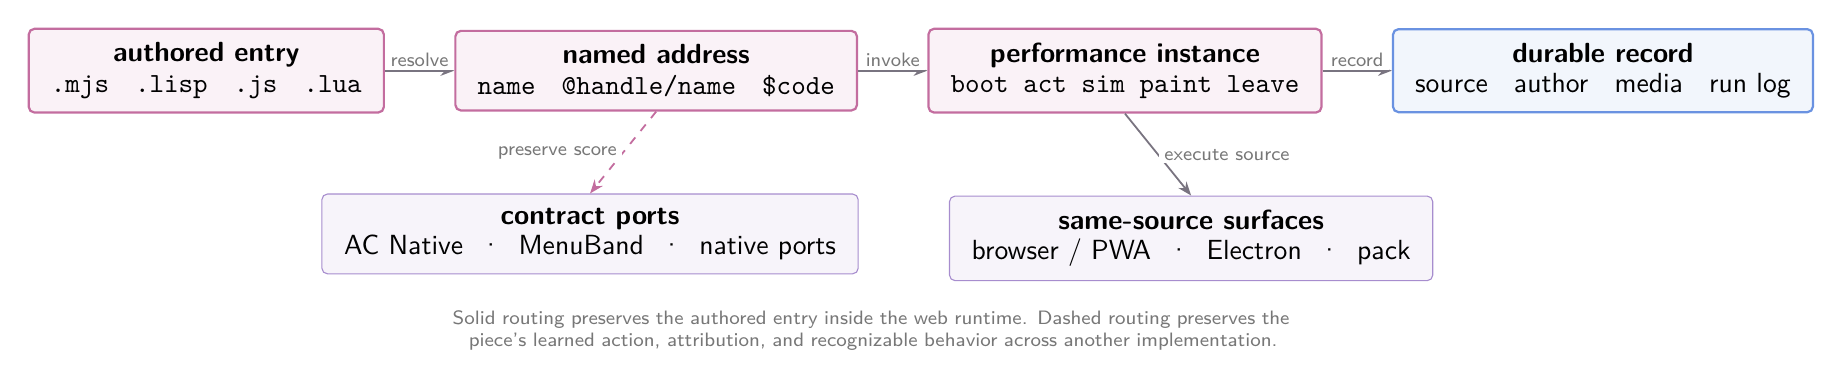
\begin{tikzpicture}[
  node distance=0.95cm and 0.88cm,
  every node/.style={font=\sffamily},
  box/.style={draw=acgray!55, rounded corners=2pt, fill=white,
    minimum height=0.92cm, align=center, inner xsep=8pt, inner ysep=5pt},
  core/.style={box, draw=acpink!80, fill=acpink!7, line width=0.8pt,
    minimum width=3.18cm},
  surface/.style={box, draw=acpurple!65, fill=acpurple!6,
    minimum width=4.95cm},
  record/.style={core, draw=acblue!70, fill=acblue!6},
  arr/.style={-{Stealth[length=5pt]}, draw=acdark!70, line width=0.65pt},
  port/.style={arr, dashed, draw=acpink!80},
  lab/.style={font=\scriptsize\sffamily, text=acgray, fill=white,
    inner xsep=2pt, inner ysep=1pt, align=center},
  note/.style={font=\scriptsize\sffamily, text=acgray, align=center}
]
  \node[core] (entry) {\textbf{authored entry}\\[-1pt]\texttt{.mjs} \; \texttt{.lisp} \; \texttt{.js} \; \texttt{.lua}};
  \node[core, right=of entry] (address) {\textbf{named address}\\[-1pt]\texttt{name} \; \texttt{@handle/name} \; \texttt{\$code}};
  \node[core, right=of address] (run) {\textbf{performance instance}\\[-1pt]\texttt{boot act sim paint leave}};
  \node[record, right=of run] (record) {\textbf{durable record}\\[-1pt]source \; author \; media \; run log};

  \draw[arr] (entry) -- node[lab, above]{resolve} (address);
  \draw[arr] (address) -- node[lab, above]{invoke} (run);
  \draw[arr] (run) -- node[lab, above]{record} (record);

  \node[surface, below=1.04cm of address, xshift=-0.84cm] (ports) {\textbf{contract ports}\\[-1pt]AC Native \;\textperiodcentered\; MenuBand \;\textperiodcentered\; native ports};
  \node[surface, below=1.04cm of run, xshift=0.84cm] (same) {\textbf{same-source surfaces}\\[-1pt]browser / PWA \;\textperiodcentered\; Electron \;\textperiodcentered\; pack};

  \draw[port] (address.south) -- node[lab, left]{preserve score} (ports.north);
  \draw[arr] (run.south) -- node[lab, right]{execute source} (same.north);

  \node[note, below=0.34cm of ports, xshift=3.57cm, text width=12.2cm] {Solid routing preserves the authored entry inside the web runtime. Dashed routing preserves the piece's learned action, attribution, and recognizable behavior across another implementation.};
\end{tikzpicture}
}
\caption{The piece contract. An authored entry resolves to a named address; invocation creates a performance instance; attribution and observation leave a durable record. Browser, Electron, and standalone packs can execute the same source. Native implementations may preserve the contract without sharing the implementation.}
\label{fig:contract}
\end{figure*}

\subsection{Authored entry}

The entry is the smallest source artifact the runtime can resolve. Built-ins are currently \code{.mjs} or \code{.lisp}; the loader can also adapt dropped or fetched p5-style \code{.js} and Lua \code{.lua} sources. The entry may import libraries, call platform services, or coordinate server state. Its unity is editorial and addressable, not dependency-free.

\subsection{Named address}

An entry becomes a piece when the system gives it a returnable name. Built-ins occupy top-level paths; published works occupy handle namespaces; KidLisp records use compact \code{\$code} addresses. Colon parameters specialize an invocation without creating another project: \code{share:notepat} asks one piece to act on another. The prompt and URL parser accept the same notation, making a typed command a portable score~\citep{scudder2026url}.

\subsection{Performance instance}

Invocation creates a run. The module may export \code{boot}, \code{act}, \code{sim}, \code{paint}, and \code{leave}; extended hooks include \code{beat}, \code{receive}, \code{preview}, and \code{meta}. Each is optional because the runtime supplies defaults. \code{act} receives input and system events, \code{sim} advances state independently of display refresh, and \code{paint} renders when a frame is needed. The newer \code{needsPaint()} path lets a quiet piece stop redrawing until an event invalidates its image. The lifecycle is therefore a performance protocol, not a mandate to animate forever~\citep{scudder2026api}.

The API arrives by parameter injection. A function declares the capabilities it uses by destructuring them:

\begin{center}
\small\ttfamily
function paint(\{ wipe, ink, circle, screen \})
\end{center}

This signature is both a working interface and a partial dependency manifest. Graphics, sound, input, storage, networking, navigation, gamepads, camera, and system services can share one calling convention while remaining under runtime control.

\begin{figure*}[t]
\centering
\resizebox{\textwidth}{!}{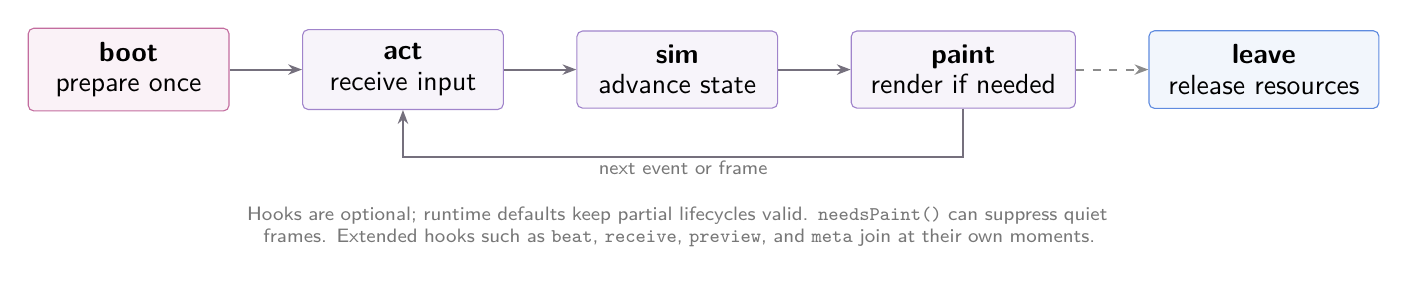
\begin{tikzpicture}[
  node distance=0.82cm and 0.92cm,
  every node/.style={font=\sffamily},
  hook/.style={draw=acpurple!70, rounded corners=2pt, fill=acpurple!6,
    minimum width=2.55cm, minimum height=0.88cm, align=center,
    inner xsep=7pt, inner ysep=5pt},
  once/.style={hook, draw=acpink!80, fill=acpink!7},
  exit/.style={hook, draw=acblue!75, fill=acblue!6},
  arr/.style={-{Stealth[length=5pt]}, draw=acdark!72, line width=0.7pt},
  opt/.style={arr, dashed, draw=acgray!85},
  lab/.style={font=\scriptsize\sffamily, text=acgray, fill=white,
    inner xsep=2pt, inner ysep=1pt, align=center},
  note/.style={font=\scriptsize\sffamily, text=acgray, align=center}
]
  \node[once] (boot) {\textbf{boot}\\[-1pt]prepare once};
  \node[hook, right=of boot] (act) {\textbf{act}\\[-1pt]receive input};
  \node[hook, right=of act] (sim) {\textbf{sim}\\[-1pt]advance state};
  \node[hook, right=of sim] (paint) {\textbf{paint}\\[-1pt]render if needed};
  \node[exit, right=of paint] (leave) {\textbf{leave}\\[-1pt]release resources};

  \draw[arr] (boot) -- (act);
  \draw[arr] (act) -- (sim);
  \draw[arr] (sim) -- (paint);
  \draw[opt] (paint) -- (leave);
  \draw[arr] (paint.south) -- ++(0,-0.62) -|
    node[lab, pos=0.25, below]{next event or frame} (act.south);

  \node[note, below=1.12cm of sim, text width=12.5cm]
    {Hooks are optional; runtime defaults keep partial lifecycles valid. \texttt{needsPaint()} can suppress quiet frames. Extended hooks such as \texttt{beat}, \texttt{receive}, \texttt{preview}, and \texttt{meta} join at their own moments.};
\end{tikzpicture}
}
\caption{The runtime lifecycle is a score with optional movements. A piece may implement only the hooks it needs; the host supplies defaults, controls repainting, and performs cleanup when the work ends.}
\label{fig:lifecycle}
\end{figure*}

\begin{figure*}[t]
\centering
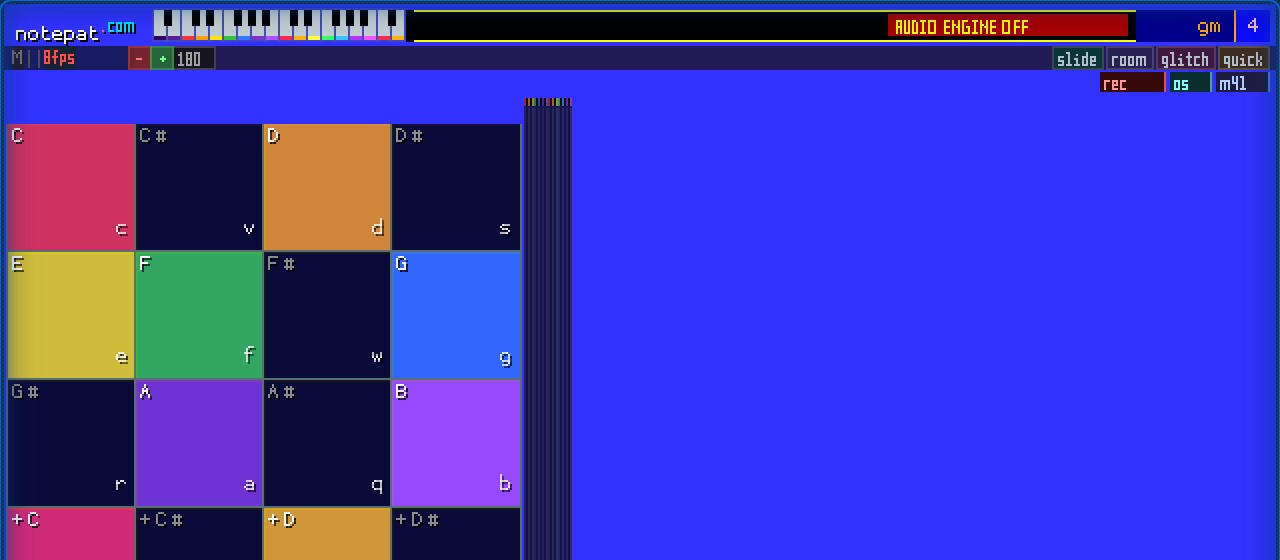
\includegraphics[width=\textwidth]{figures/ac-notepat-crop}
\caption{\code{notepat} running at \code{aesthetic.computer/notepat}, captured August 5, 2026. The address resolves directly to a performance surface; visible pitch names and QWERTY bindings make learned action part of the work.}
\label{fig:notepat}
\end{figure*}

\subsection{Durable record}

The source and its author outlive any run. Publication records, handle paths, generated previews, paintings, tapes, and source retrieval allow a piece to circulate in forms other than a live tab. Since 2026, each load also receives a fresh \code{pieceId}; the runtime batches console events and records start, log, error, and completion phases in an admin-readable collection. A run is evidence about a piece, not the piece itself.

This separation aligns the piece with the \emph{versioned virtual object} developed in the companion Keymaps paper: identity persists through multiple implementations and revisions because a community continues to treat them as the same thing~\citep{scudder2026keymaps}. The named work is the continuity claim; source and runs are its versions and performances.

\section{Evidence from the Monorepo}

The repository census in Table~\ref{tab:census} was computed from the checked-out source on August 4, 2026. The method and raw counts live beside the paper in \code{data/monorepo-snapshot.json}. These are source facts, not production analytics.

\begin{table*}[t]
\small
\centering
\begin{tabularx}{\textwidth}{l r X}
\toprule
\textbf{Measure} & \textbf{Count} & \textbf{What it establishes} \\
\midrule
Built-in entry files & 477 & 455 JavaScript modules and 22 KidLisp files in \code{disks/}. \\
JavaScript entries with imports & 188 & The entry-file boundary does not imply a self-contained implementation. \\
Exporting \code{boot} / \code{paint} & 381 / 381 & Most JavaScript entries opt into the visible start-and-render protocol. \\
Exporting \code{act} / \code{sim} & 316 / 248 & Interaction is more common than fixed-step simulation; neither is required. \\
Exporting \code{leave} / \code{beat} & 80 / 27 & Cleanup and metrical time are explicit specialized hooks. \\
Exporting \code{meta} / \code{receive} & 194 / 18 & Discoverability and inter-piece messaging are opt-in layers. \\
JavaScript length, median / 90th pct. & 152 / 762 & A compact center coexists with a long tail; the largest entry is about 10k lines. \\
Top-level library modules / server functions & 96 / 163 & The piece corpus sits inside substantial shared and operational infrastructure. \\
\bottomrule
\end{tabularx}
\caption{Syntactic census of the August 4, 2026 monorepo at commit \code{c65015fe25}. Hook counts detect top-level export lines and do not measure how often a hook runs.}
\label{tab:census}
\end{table*}

The counts support three narrower claims.

First, the lifecycle is a family resemblance, not a schema every work must fill. Both \code{boot} and \code{paint} appear in 381 JavaScript entries; \code{beat} appears in 27 and \code{receive} in 18. Runtime defaults make partial participation valid. A static score, a networked game, and a musical tool can remain pieces without exporting the same hooks.

Second, the corpus has outgrown the sketch-sized implementation without abandoning the sketch-sized entry. The median JavaScript entry is 152 lines, but the ninetieth percentile is 762 and the largest is about 10,000. Shared engines let related works remain distinct at the address layer. The July 2026 \code{pads} family is illustrative: many named audiovisual instruments import one engine, while each entry supplies its own palette, voice, and behavior.

\code{dannom.mjs} makes the same point at a smaller scale. Its 19-line entry fixes a Danish language mode and re-exports lifecycle functions from the shared \code{nom.mjs} engine. The compact source is real, but it belongs to the authored-entry layer rather than describing the size of the performed system.

\begin{figure*}[p]
\centering
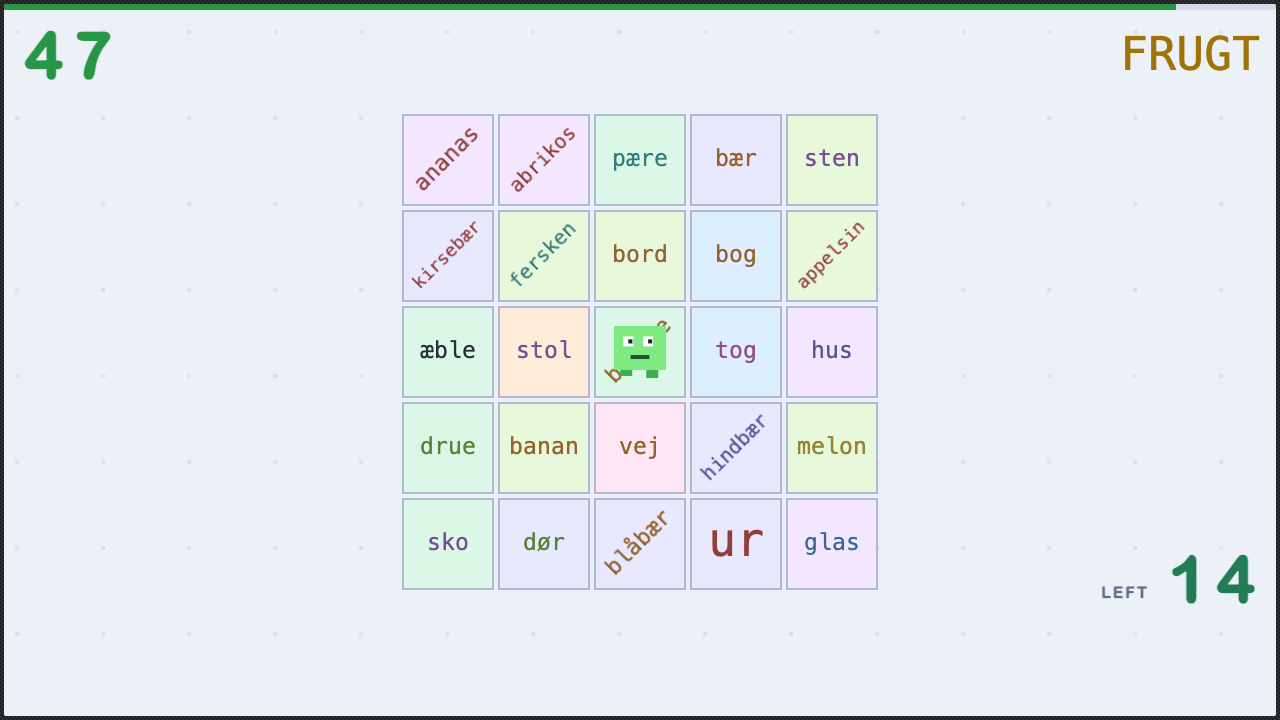
\includegraphics[width=0.90\textwidth]{figures/ac-dannom-play}\par
\vspace{0.65em}
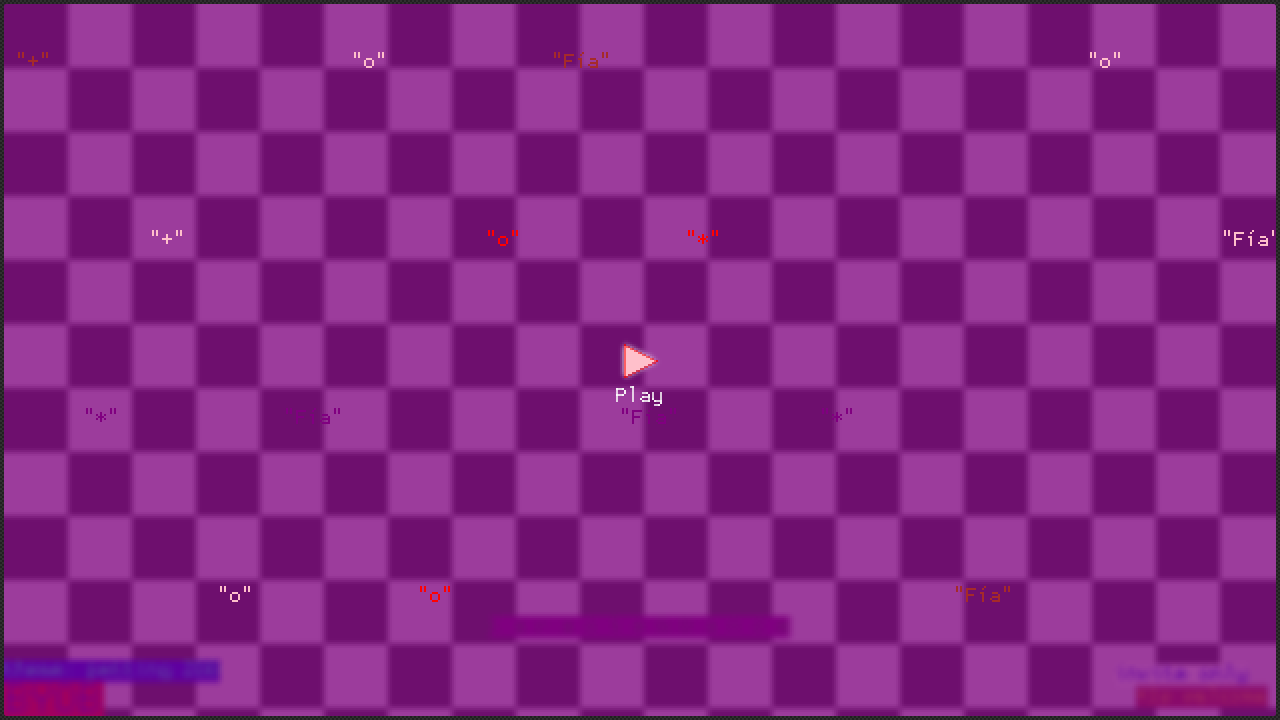
\includegraphics[width=0.90\textwidth]{figures/ac-kidlisp-fia-birthday-live}
\caption{Small entries can open substantial performance surfaces. Top: \code{dannom}, a Danish edition over the shared \code{nom.mjs} game engine. Bottom: \code{fia-birthday}, one of 22 built-in KidLisp entries. Both were captured from their public addresses on August 5, 2026.}
\label{fig:entry-surfaces}
\end{figure*}

Third, the corpus changes faster than a paper can. The Research Platter last synchronized on July 21 listed 413 built-in pieces, 88 library modules, and 126 server functions~\citep{acplatter2026}. Two weeks later the checkout contained 477 entries, 96 libraries, and 163 functions. The gap is not an error to smooth away. It is evidence that publication needs dated provenance.

\section{Address and Composition}

\subsection{A path is a public score}

The path \code{notepat} is short enough to say aloud, type from memory, print as a QR, or embed in another piece. URL addressability turns invocation into notation. The prompt is not merely a launcher layered over a project system; it is another interpreter for the same names the web already routes~\citep{scudder2026url}. This makes the piece social before anyone opens its source.

Steyerl's ``poor image'' gains force by circulating in degraded copies~\citep{steyerl2009poor}. A piece faces the opposite problem: it needs a runtime, input, and time. The named address is the compression that lets this richer object circulate without reducing it to a screenshot. The path travels cheaply; the encounter rehydrates at the destination.

\begin{figure*}[t]
\centering
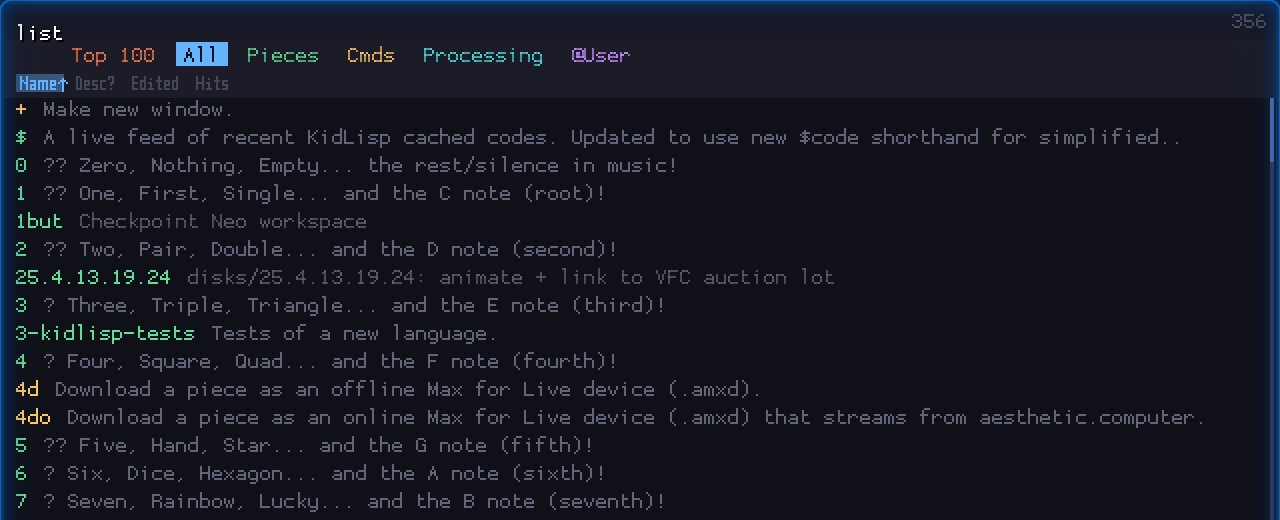
\includegraphics[width=\textwidth]{figures/ac-list-crop}
\caption{The public \code{list} piece, captured August 5, 2026. Names and one-line descriptions turn the built-in corpus into a navigable repertoire rather than a directory of implementation files.}
\label{fig:list}
\end{figure*}

\subsection{Publishing makes a claim of authorship}

Registered authors publish beneath a chosen handle. \code{source name} exposes a starting point for revision; the new work can receive another name and author. The musical metaphor of a \emph{cover} is useful only if provenance remains visible. Otherwise it romanticizes copying. In practice, the system needs both operations: source-level forking for technical lineage and naming/attribution for cultural lineage.

The July 21 Platter snapshot recorded 2,810 handles, 265 user-published JavaScript pieces, 4,425 paintings, 16,523 KidLisp programs, and 18,048 chat messages~\citep{acplatter2026,scudder2026network}. These categories should not be collapsed. A built-in entry, a published JavaScript work, a compact KidLisp code, a painting, and a chat utterance have different storage and governance. They meet at the prompt because the prompt can address each one.

\code{@sat} shows a handle acting as a returnable portfolio rather than a generic account row. \code{laer-klokken} shows the complementary community boundary: its original address now aliases \code{laklok}, while the live room remains reachable under the name its participants know.

\begin{figure*}[p]
\centering
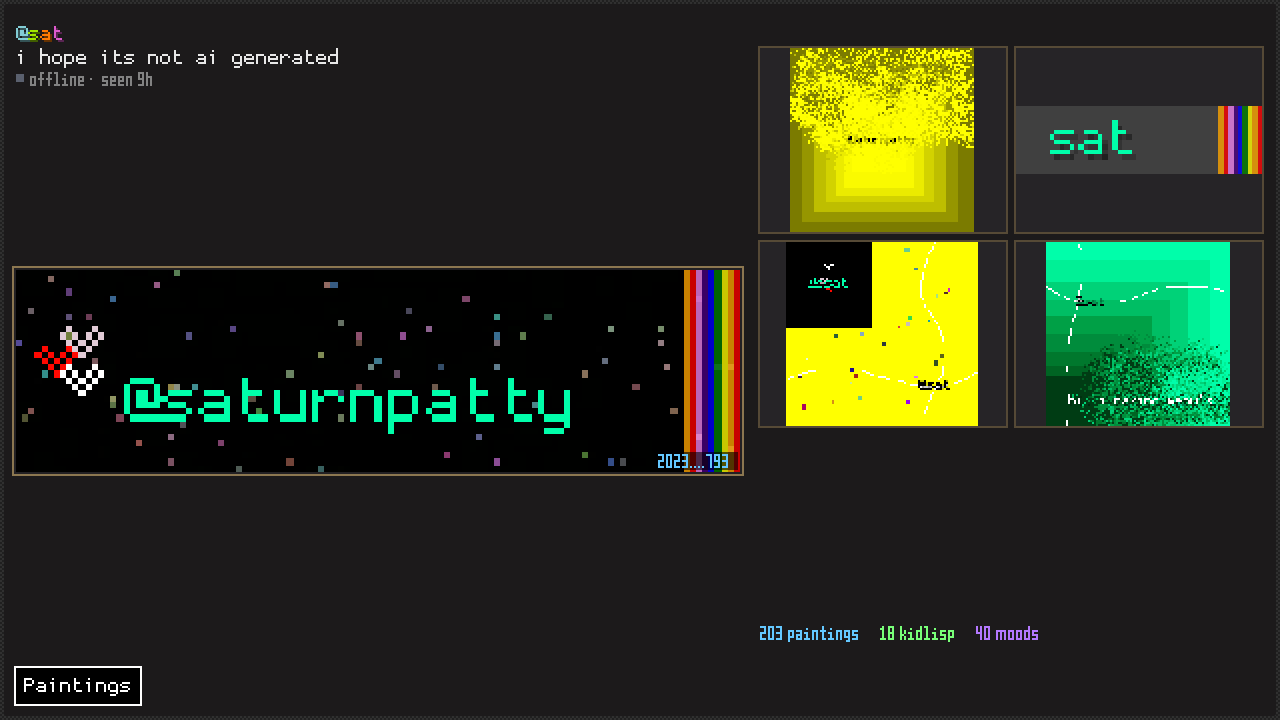
\includegraphics[width=0.90\textwidth]{figures/ac-profile-sat-live}\par
\vspace{0.65em}
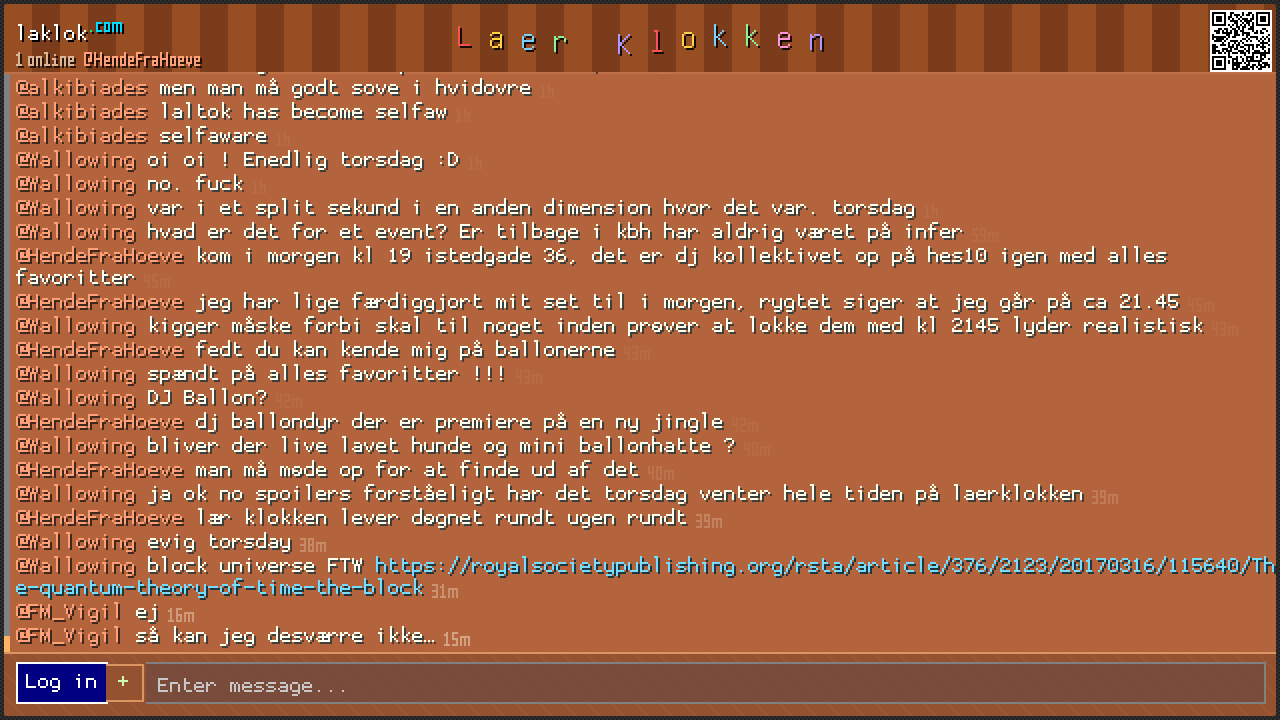
\includegraphics[width=0.90\textwidth]{figures/ac-laer-klokken-live}
\caption{Addresses join works to people and communities. Top: \code{@sat}'s public profile gathers paintings, KidLisp works, and moods under one designed handle. Bottom: the signed-out public \code{laer-klokken} room preserves an established name while its entry delegates to \code{laklok}. Captured August 5, 2026.}
\label{fig:social-addresses}
\end{figure*}

\subsection{The piece is composable, not total}

The feature set now includes units above and beside pieces. A \code{\^bag} is an admin-curated container mixing pieces, KidLisp codes, paintings, and tapes. Prompt conductors can expand \code{\^pads} into a sequence of constituent works. A development \code{channel} broadcasts incremental source changes to several devices. Multiplayer pieces such as \code{arena} coordinate a browser entry with authoritative server logic. These are not failures of the piece model. They show where its boundary ends.

The piece is the unit one can invoke and attribute. A bag is a collection; a channel is a rehearsal route; a session is a shared performance; a server is an authority. Treating all four as ``the piece'' would erase useful architecture. Treating none of them as part of the work would erase the conditions of performance.

\begin{figure*}[t]
\centering
\resizebox{0.86\textwidth}{!}{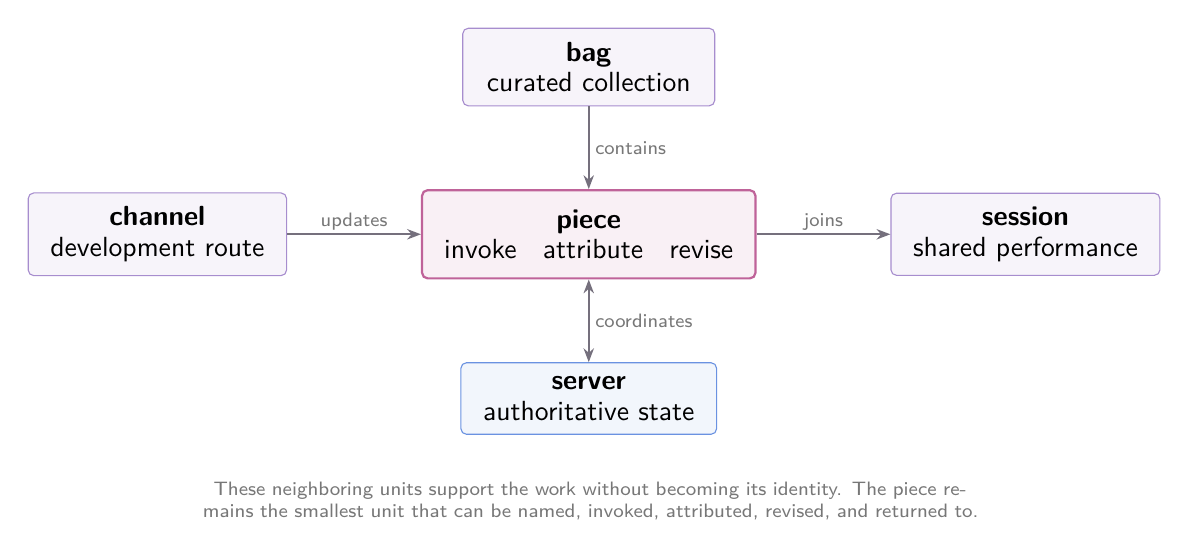
\begin{tikzpicture}[
  node distance=1.0cm and 1.55cm,
  every node/.style={font=\sffamily},
  core/.style={draw=acpink!85, rounded corners=2pt, fill=acpink!8,
    minimum width=3.35cm, minimum height=1.12cm, align=center,
    inner xsep=8pt, inner ysep=5pt, line width=0.8pt},
  neighbor/.style={draw=acpurple!65, rounded corners=2pt, fill=acpurple!6,
    minimum width=3.2cm, minimum height=0.9cm, align=center,
    inner xsep=8pt, inner ysep=5pt},
  authority/.style={neighbor, draw=acblue!70, fill=acblue!6},
  arr/.style={-{Stealth[length=5pt]}, draw=acdark!72, line width=0.7pt},
  back/.style={{Stealth[length=5pt]}-{Stealth[length=5pt]}, draw=acdark!72,
    line width=0.7pt},
  lab/.style={font=\scriptsize\sffamily, text=acgray, fill=white,
    inner xsep=2pt, inner ysep=1pt, align=center},
  note/.style={font=\scriptsize\sffamily, text=acgray, align=center}
]
  \node[core] (piece) {\textbf{piece}\\[-1pt]invoke \; attribute \; revise};
  \node[neighbor, above=1.05cm of piece] (bag) {\textbf{bag}\\[-1pt]curated collection};
  \node[neighbor, left=1.7cm of piece] (channel) {\textbf{channel}\\[-1pt]development route};
  \node[neighbor, right=1.7cm of piece] (session) {\textbf{session}\\[-1pt]shared performance};
  \node[authority, below=1.05cm of piece] (server) {\textbf{server}\\[-1pt]authoritative state};

  \draw[arr] (bag) -- node[lab, right]{contains} (piece);
  \draw[arr] (channel) -- node[lab, above]{updates} (piece);
  \draw[arr] (piece) -- node[lab, above]{joins} (session);
  \draw[back] (piece) -- node[lab, right]{coordinates} (server);

  \node[note, below=0.48cm of server, text width=12.8cm]
    {These neighboring units support the work without becoming its identity. The piece remains the smallest unit that can be named, invoked, attributed, revised, and returned to.};
\end{tikzpicture}
}
\caption{A piece sits beside other named operational units. Bags contain pieces, channels update them, sessions coordinate shared runs, and servers may own authoritative state; none replaces the piece as the unit of address and attribution.}
\label{fig:ecology}
\end{figure*}

\section{Across Substrates}

The web runtime remains the canonical execution surface. The same entry can run in a browser or PWA, inside the Electron application's webview, or inside a generated standalone pack. These are source-preserving distributions: the adapter and host change, while the entry executes as written.

AC Native introduces a second relation. Its QuickJS/C environment implements a compatible creative-computing surface on bare metal, but not every web piece runs unchanged and some works have purpose-built native implementations~\citep{scudder2026os}. \code{notepat}, for example, exists as a browser piece, a native instrument, a macOS menubar instrument, and other ports. The Keymaps paper shows that its input mapping is the cross-substrate contract~\citep{scudder2026keymaps}; the present paper extends that observation. A piece can survive a port when its name, interaction score, and recognizable behavior survive, even when the code does not.

This yields a practical test: two implementations count as performances or ports of one piece when a returning participant can carry learned action, expectation, and attribution from one to the other. Shared source is sufficient, not necessary. The test is social and contestable. It prevents a brand label alone from declaring equivalence while allowing a work to cross hardware boundaries.

\section{Trust, Cleanup, Observation}

An artistic name does not suspend software's risks. Ruha Benjamin's account of discriminatory design is a warning against treating humanized language as evidence of humane infrastructure~\citep{benjamin2019race}. The piece model therefore has to state who may do what, what survives a run, and what the operator records.

\subsection{Capability boundaries}

Built-in entries are trusted. User-uploaded JavaScript receives a restricted API that namespaces storage, blocks authentication tokens, and requests permission before API-mediated network access, external upload, or navigation. KidLisp is constrained by language design: it omits general file, network, and string facilities~\citep{scudder2026kidlisp}. This is a useful capability boundary, but it is not a complete sandbox. Static imports and browser globals require their own threat model. The honest claim is narrower: injected capabilities make sensitive operations visible and mediatable; they do not prove containment.

\subsection{Leaving is part of performing}

Only 80 JavaScript entries explicitly export \code{leave}, so the host also performs global cleanup when switching pieces. Both layers matter. A musical or camera piece can leave audio nodes, media tracks, timers, or session membership behind if teardown is treated as an afterthought. \code{leave} is the formal end of a performance; host cleanup is the safety net when the performer fails.

\subsection{Run logs create obligations}

Piece-run telemetry stores a slug, boot identifier, host, user agent, approximate geography from request headers, console events, errors, and completion summaries. Reads are admin-gated and event arrays are capped, but the contents can still include accidental personal data. This paper uses only the public schema and no raw run records. A mature piece model needs retention limits, disclosure, and a way to keep private creative work from becoming operational exhaust. Observability makes maintenance possible; minimization keeps the maintenance system from becoming another audience.

\section{Design Consequences}

The contemporary feature set replaces five romantic slogans with narrower contracts:

\begin{enumerate}
  \item \textbf{One addressable entry, not one implementation file.} Imports and server companions are allowed; the public boundary stays small.
  \item \textbf{A lifecycle with defaults.} Hooks describe moments of performance, and pieces opt into only the moments they need.
  \item \textbf{Capabilities are passed, not presumed.} Injection supports documentation, testing, and partial restriction.
  \item \textbf{Names carry attribution and return.} Paths, handles, source retrieval, previews, and media records preserve continuity beyond a run.
  \item \textbf{Composition uses explicit neighboring units.} Bags, channels, sessions, and ports should name their own contracts instead of disappearing inside ``piece.''
\end{enumerate}

The shift also changes evaluation. A program can be tested for correctness without asking whether anyone can find it again. A piece needs both technical and cultural tests: Does it boot and leave cleanly? Does input remain learnable across revisions? Is its address stable? Is its author visible? Can a participant return without relearning the work? Does a port preserve the score or only the logo?

\section{Limitations}

This is a situated account of one monorepo, most of whose built-in corpus has one primary author. It cannot show that calling software \emph{pieces} causes a practice culture; the architecture, community, and vocabulary developed together. Hook counts are syntactic and do not measure runtime use. Platter adoption figures are a July 21 snapshot rather than a new production query. No demographic or raw telemetry data was inspected.

The prompt's memorizable namespace also has an accessibility cost: a path is easy only after someone learns it. Lists, autocomplete, metadata, documentation, and direct links remain necessary. Only 194 of 455 JavaScript entries export \code{meta}; curated documentation partly fills the gap, but reachability is not discoverability.

Finally, the piece concept can overstate autonomy. Sadie Plant's history of computing makes visible how apparently singular artifacts emerge from distributed, gendered technical labor~\citep{plant1997zeros}. A named author and entry file should not hide browser standards, library maintainers, server operators, hardware, energy, or community knowledge. The piece is a useful unit of address and analysis, not the only unit that matters.

\section{Conclusion}

``Pieces not programs'' is not a demand to stop engineering. It is a demand to engineer for a work that must survive more than execution. In the current \ac{} monorepo, a piece is an authored entry, a named address, a lifecycle-governed performance, and a durable record. It can be 30 lines or 10,000; self-contained or backed by libraries and services; executed from the same source or carried across substrates by a behavioral contract.

The contemporary evidence strengthens the artistic claim by removing its weakest literalism. The piece is not one file. It is the smallest work the system can name, invoke, attribute, revise, and return to. Programs make it run. Practice makes it persist.

\bibliographystyle{plainnat}
\setlength{\bibsep}{1.2pt plus 0.2ex}
\onecolumn
\begin{multicols}{2}
{\footnotesize
\bibliography{references}
}
\end{multicols}

\vspace{0.8em}
\begin{center}
\footnotesize\sffamily\color{acgray}
Revision \paperrev\;\textperiodcentered\;\texttt{\paperhash}\;\textperiodcentered\;
\href{https://papers.aesthetic.computer/pieces-not-programs-26-arxiv.pdf}{papers.aesthetic.computer/pieces-not-programs-26-arxiv}
\end{center}

\end{document}
